\selectlanguage{spanish}
\let\textcircled=\pgftextcircled
\chapter {Introducción}
\label{chap:intro}

\initial{E}l tráfico urbano es uno de los principales retos a los que se enfrentan las ciudades. El mundo se urbaniza rápidamente y la densidad de población aumenta. Este crecimiento conlleva una expansión de la demanda y ha llevado a priorizar la aplicación de estrategias que permitan disminuir la congestión global. Estas técnicas se ubican en tres áreas principales: gobierno, optimización de la red de transporte y servicios de transporte integrados, en este último se ubican los sistemas de información al viajero que proveen información en tiempo real. 

Sin embargo, dentro de las áreas mencionadas, no es posible llevar a cabo estrategias si no se conocen las variables que describen el estado real del sistema: densidad de ocupación, flujo vehicular y velocidades medias. Para obtener estos datos existen productos comerciales, como Mistic de Swarco y CitySolver de Bitcarrier, pero estos requieren elevados costos de instalación y mantenimiento. Para las autoridades, es indispensable contar con información del estado de la red ya que permite tomar decisiones fundamentadas para mejorar las condiciones de tráfico y así mejorar la calidad de vida de los habitantes.

\section{Motivación}
\label{sec:motivacion}

En lo que refiere a los sistemas de transporte, la mayoría de los líderes gubernamentales coinciden en que es necesario invertir en infraestructuras. Sin embargo, las restricciones impuestas por la limitación presupuestaria obligan a gestionar más eficazmente la demanda y el suministro mediante el despliegue de sistemas de transporte inteligente (ITS) \cite{transpinteligente2009}. 
El crecimiento del parque automotor a nivel mundial, también registrado en Argentina\cite{ondat2015}, repercute directamente en el aumento del nivel de congestión vehicular\cite{de1994modelling}. Según un estudio realizado mundialmente, en Buenos Aires la cantidad media de paradas-arranques realizadas por vehículo por año asciende a 23.760 \cite{castrol2014}, lo que revela el aumento de los períodos de viaje ociosos, es decir, demoras en atascos, semáforos, etc. Asimismo, una encuesta realizada por IBM, conocida como ``Commuter Pain Index'' (índice de dolor del viajero),  sitúa a Buenos Aires entre las ciudades con peor tráfico a nivel mundial, por encima de mega-ciudades como París y Los Ángeles (\ref{fig:commuter-pain-index}). Aquí se observaron otros aspectos además de las paradas-arranques;  al cabo de 1 año se volvió a encuestar a los viajantes y en el caso de la ciudad de Buenos Aires, un 41\% cambió al transporte público por los aumentos en los costos económicos. No menos preocupante es la cantidad de viajes cancelados reportados por los conductores, en donde un 43\% de ellos corresponden a viajes de trabajo. Finalmente cabe destacar que el 44\% manifestó haber sufrido algún trastorno de salud (principalmente estrés) a causa del tráfico.

En cuanto a los costos que implica la congestión, la operación de los vehículos que circulan en las vías de ciudades de más de 100.000 habitantes consume alrededor del 3.5\% del PBI de América Latina y el Caribe\cite{bull2003congestion}. Por ende, es notable la necesidad de contar con herramientas que permitan a las autoridades aplicar políticas para mejorar las condiciones del transporte.

\begin{figure}[!htp]
\centering
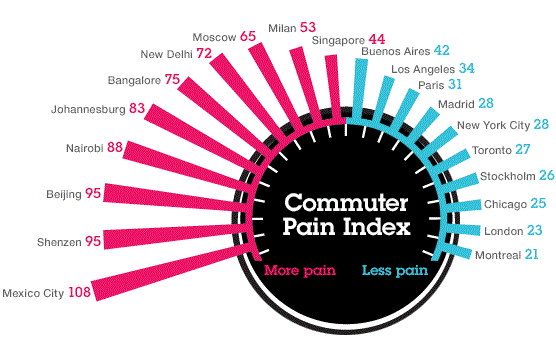
\includegraphics[width=0.6\textwidth]{images/commuter-pain-index.png}
\captionsetup{width=0.6\textwidth}
\caption{Ranking de ciudades con peor trafico en el mundo ``Commuter Pain Index'' (IBM 2011)}
\label{fig:commuter-pain-index}
\end{figure}

Resolver estos problemas depende de planificaciones urbanas que aseguren un sistema operacional y económicamente eficiente. Para planificar, es indispensable contar con registros históricos del estado de la red a lo largo del tiempo para la toma de decisiones. La actividad vehicular puede ser detectada a partir de distintos tipos de fuentes, tradicionalmente, por cámaras de video, detectores infrarrojos (Figura \ref{fig:IRDetector}) y bucles de inducción (ó \textit{induction loops}, Figura \ref{fig:ILDetector}). Si bien se trata de métodos precisos, son costosos y requieren la instalación del equipamiento sobre los caminos, dificultando el despliegue sobre varios puntos de una ciudad.

Por otro lado, la incorporación de dispositivos de tecnología inalámbrica Wi-Fi y Bluetooth en automoviles particulares, lleva a nuevas formas de obtener datos de la movilidad urbana realizando capturas de los vehículos en tránsito, permitiendo inferir su ubicación. Este mecanismo de recolección de datos se considera no invasivo ya que no es necesario alterar la vía para su instalación, como en el caso de los detectores por inducción magnética. Esto lo convierte en un método de bajo costo y fácil instalación, con posibilidad de ser extendido a múltiples aplicaciones, como por ejemplo: posicionamiento en interiores basado en señales Wi-Fi\cite{jekabsons2011analysis} y análisis de uso de líneas de autobuses en base a seguimiento de usuarios vía Wi-Fi y Bluetooth\cite{dunlap2016estimation}. 

\begin{figure}[!htb]
\centering
\begin{minipage}{.45\textwidth}
%{15.5cm}
    \centering
    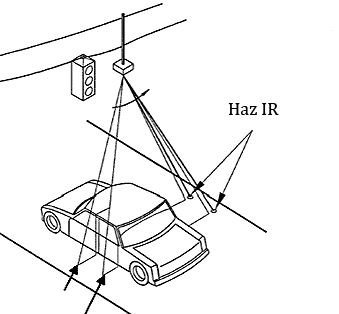
\includegraphics[height=0.2\textheight]{images/detector-infrarrojo.png}
    \caption {Detectores infrarojos}
    \label{fig:IRDetector}  
\end{minipage}
\begin{minipage}{.45\textwidth}
%{15.5cm}
    \centering
    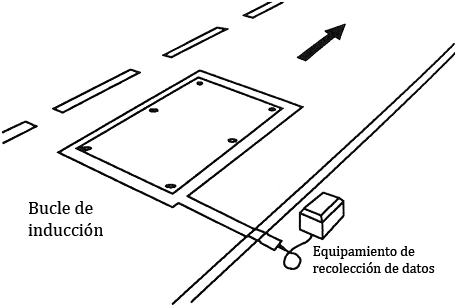
\includegraphics[height=0.2\textheight]{images/detector-inductionloop.png}
    \caption {Bucles de inducción}
    \label{fig:ILDetector}  
\end{minipage}
\end{figure}

La naturaleza estocástica de las transmisiones recolectadas presenta un desafío significativo respecto a su interpretación. Trabajos previos\cite{lou2009map,thiagarajan2009vtrack,wei2012fast} demuestran que es posible inferir trayectorias a partir de observaciones escasas y ruidosas aplicando cadenas ocultas de Markov y su decodificación a través del algoritmo de Viterbi.

En el siguiente trabajo se utiliza el algoritmo de “Viterbi” sobre modelos ocultos de Markov aplicado a la estimación de estados y tiempos de viaje en redes de tráfico a partir de señales de GPS y Bluetooth. El método a desarrollar está basado en la estimación de la velocidad media espacial a partir de la trayectoria de los vehículos. 

\section{Trabajos relacionados}
\label{sec:trabajosrelacionados}
En el marco del proyecto ``Estimación del estado del tráfico vehicular a través de datos obtenidos de dispositivos móviles'', del programa ``Universidad y Transporte Argentino'',  se desarrolló un prototipo para censar y realizar seguimiento de vehículos. La solución cuenta con tres técnicas de captura de datos: localización geográfica a partir de lecturas de GPS, registro de dispositivos Bluetooth cercanos a un detector y conteo vehicular a través de videocámaras. El prototipo permite el envío de las observaciones obtenidas a un servidor central para su procesamiento. 

Las técnicas mencionadas anteriormente se implementan en dos módulos separados: una aplicación Android para dispositivos con sensor GPS, y dos cajas sensores denominadas ``C3P0'' y ``R2D2'' (Figura \ref{fig:c3p0}). Estas cajas realizan las mismas funciones: por un lado, realizan un conteo de vehículos que circulan por un determinado punto de la red a partir del procesamiento de video, y por otro, registran lecturas de la señal de radiofrecuencia emitida por dispositivos Bluetooth activos. En las cajas se utilizan dispositivos Ubertooth One\cite{ossmann2012project}, estos son dispositivos USB con conectividad Bluetooth a través del microchip CC2400. Este chip posee un transceptor que permite monitorear transmisiones Bluetooth y, a partir del software que acompaña al dispositivo, se registran características de los paquetes capturados, como identificación del dispositivo de origen, nivel de señal de la transmisión, marcas temporales, etc. Por ejemplo en la Figura \ref{fig:ubertooth-capture} se muestra en funcionamiento la herramienta de captura, en donde se observa un vehículo y su señal interceptada.

\begin{figure}[!htp]
\centering
\captionsetup{width=.9\linewidth}
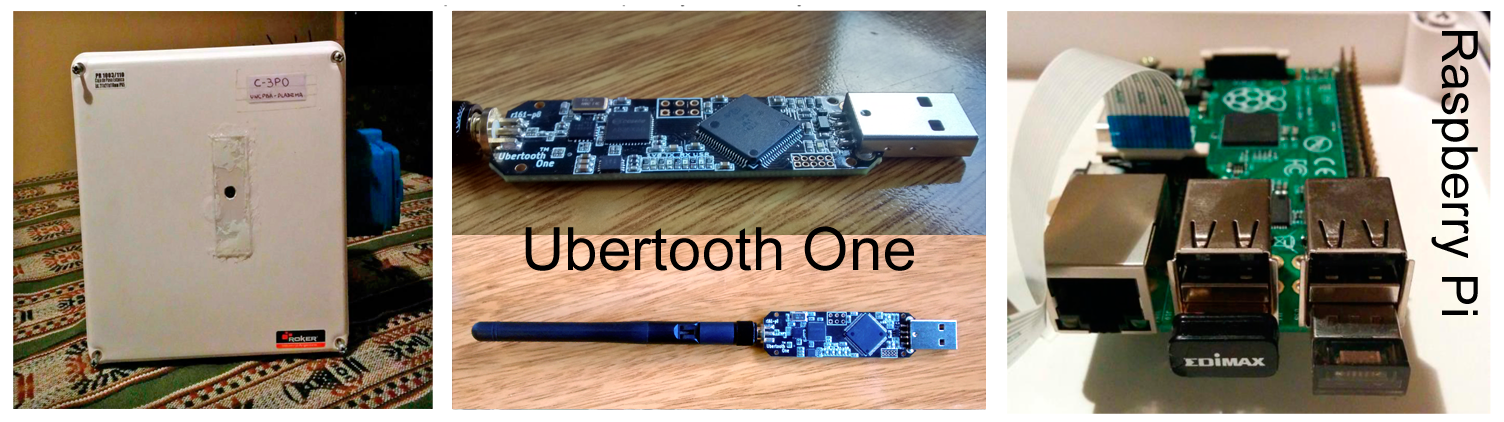
\includegraphics[width=0.9\linewidth]{images/c3p0.png}
\caption{Las cajas ``C3P0'' y ``R2D2'', son construidas con una Raspberry Pi, una cámara de 5 MP , un dongle Wi-Fi para armado de la red ad-hoc y un dispositivo Ubertooth One para la captura de señales. }
\label{fig:c3p0}
\end{figure}

Las cajas pueden ser accedidas a través de un sitio web en una red ad-hoc, para monitorizar su funcionamiento y configurar los parámetros de recolección y reporte de datos. Cabe mencionar que el prototipo fue construido sobre una caja estanca para poder ser ubicado a la intemperie.

Como se mencionó, esta metodología considera métodos no invasivos, algo que comparte con algunos productos comerciales. Se utiliza tecnología Bluetooth porque permite identificar unívocamente un vehículo. Además, es mas probable encontrar vehículos con Bluetooth integrado que una gran de usuarios utilizando una aplicación determinada.

\begin{figure}[!htp]
\centering
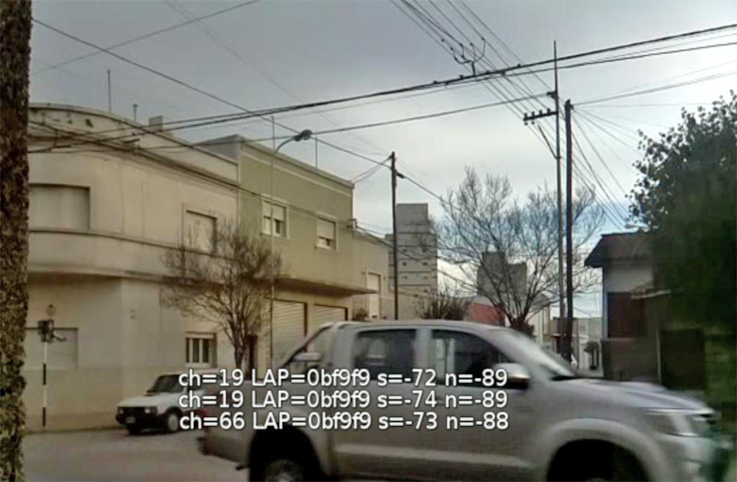
\includegraphics[width=0.7\textwidth]{images/ubertooth-capture.png}
\captionsetup{width=.7\linewidth}
\caption{Captura obtenida de la caja ``R2D2'' detectando paquetes de un mismo dispositivo (misma LAP).}
\label{fig:ubertooth-capture} 
\end{figure}

Por último, se aclara que en el presente trabajo se utilizan desarrollos realizados en otro proyecto final de grado dentro del área de tráfico vehicular, en donde se desarrolló un software que conecta dos herramientas para la simulación de tráfico: un editor de mapas de Open Street Map (JOSM) y un simulador de tráfico microscópico (SUMO).

\section{Sistemas de comunicación inalámbricos}

Aquí no se pretende ser extenso sobre los fenómenos físicos que dan lugar al comportamiento de los canales inalámbricos. En su lugar, se mencionan conceptos que hacen a la problemática del uso de estos dispositivos como fuente de información. Si el lector lo requiere, podrá consultar mayores detalles en \cite{aragon2008antennas}.

\begin{figure}[!htp]
\centering
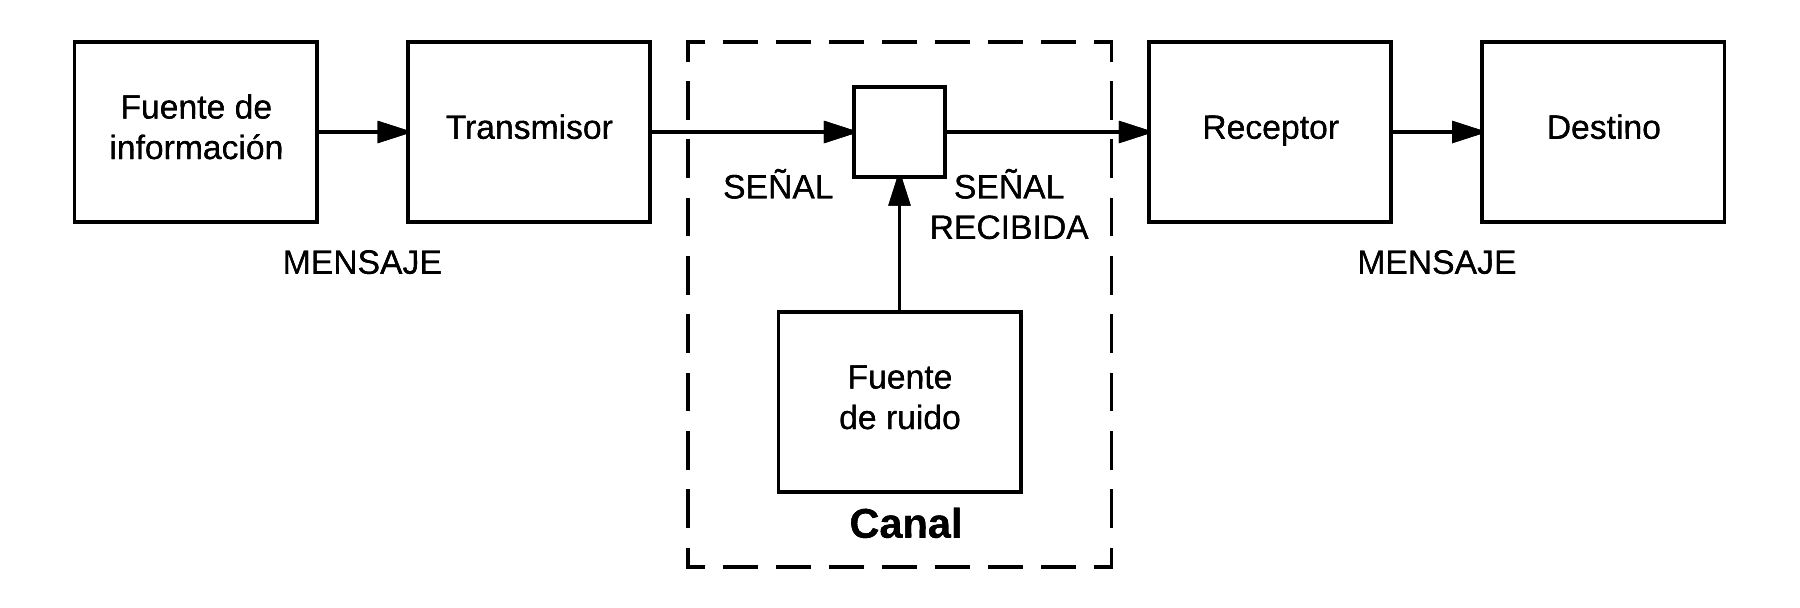
\includegraphics[scale=0.9]{images/comm-system.png}
\caption{Esquema general de un sistema de comunicaciones}
\label{fig:comm-system}
\end{figure}

La arquitectura genérica de un sistemas de comunicaciones, ilustrada por la Figura \ref{fig:comm-system}, fue presentada originalmente por Claude Shannon\cite{shannon2001mathematical}. Ya sea para sistemas alámbricos o inalámbricos, un \textit{canal} es el medio sobre el cual se transmite la señal generada por un transmisor destinada a un receptor. 

%El transmisor convierte datos de una fuente de información (ej. un teléfono móvil) en una señal acorde para ser enviada a través del canal. El canal mismo modifica la señal en diferentes formas por lo que el receptor debe estar diseñado para salvar estas alteraciones y reproducir el mensaje con el menor error posible. 

El recurso básico utilizado en las comunicaciones inalámbricas es el espectro electromagnético. En general, para comunicaciones se utilizan frecuencias entre 3 kHz y 300 GHz, que corresponden a longitudes de onda en el espacio abierto desde 100 km a 1 mm. A mayor frecuencia, mayor es el ancho de banda disponible.  Los sistemas Bluetooth funcionan en la banda ISM (Industrial, Científica y Médica) de los 2.4 GHz, liberada por la UIT (Unidad Internacional de Telecomunicaciones).

El diseño de una antena establece algunos de los efectos y características que tendrá la señal transmitida. El propósito es asegurar mejor eficiencia en la transmisión, con antenas que irradian mayor energía en dirección al receptor. Para representar la distribución tridimensional de energía radiada se utiliza el patrón de radiación. Este define la variación de la potencia irradiada por una antena como función de la posición relativa a la misma. El ejemplo más simple es el de una antena ideal que irradia igualmente en todas las direcciones: la antena isotrópica (Figura \ref{fig:antenna-pattern})

\begin{figure}[!htp]
\centering
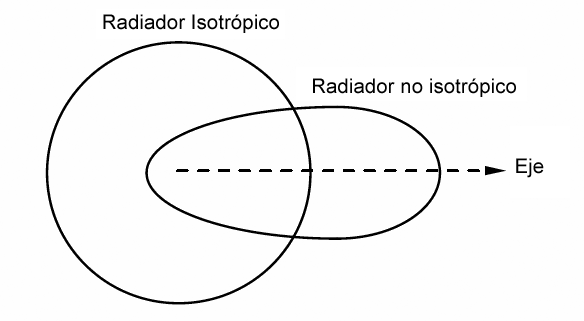
\includegraphics[scale=0.4]{images/isotropic_radiator.png}
\captionsetup{width=.6\linewidth}
\caption{Esquema de radiación de una antena isotrópica y una antena direccional}
\label{fig:antenna-pattern}
\end{figure}

Desde un punto de vista de un único transmisor, la atenuación de señal es el factor limitante del rango de transmisión efectivo\cite{schmidt2009degradation}. El desarrollo de modelos para propagación de señales es realizado generalmente usando valores estadísticos de regiones o ciudades en particular. Los modelos de atenuación, conocidos como ``Path Loss'', permiten calcular la atenuación de señal o la potencia de señal recibida para una distancia dada entre emisor y receptor. Además de la atenuación debida a la propagación sobre el aire, existen otros factores que afectan la transmisión:

\begin{itemize}
  \item Reflexión: Las ondas electromagnéticas son reflejadas por varias superficies. En el caso de comunicaciones a gran distancia, el hielo es la superficie que mejor refleja la señal, seguido por las acumulaciones de agua y los terrenos húmedos. En el caso opuesto, las superficies áridas son las que menos reflejan. A corta distancia, la reflexión se da en edificios, en especial aquellos con superficies metálicas. Como resultado se tienen señales viajando a través de múltiples caminos.
   \item Oscurecimiento \textit{(Shadowing)}: Algunos objetos reflejan las ondas en dirección opuesta o atenúan fuertemente la señal de modo que sólo permanecen señales débiles detrás de estos objetos.
   \item Difracción: La onda se dobla sobre bordes pronunciados de un objeto. Así, la onda es capaz de propagarse mas allá de los objetos que producen \textit{shadowing} (Figura \ref{fig:shadowing}).
   \item Dispersión \textit{(Scattering)}: Al contrario de la reflexión que ocurre en superficies relativamente amplias, la dispersión se da en pequeñas superficies en comparación a la longitud de onda. Superficies ásperas como plantas y árboles dispersan la onda en múltiples direcciones.
\end{itemize}

\begin{figure}[!htp]
\centering
\captionsetup{width=.7\linewidth}
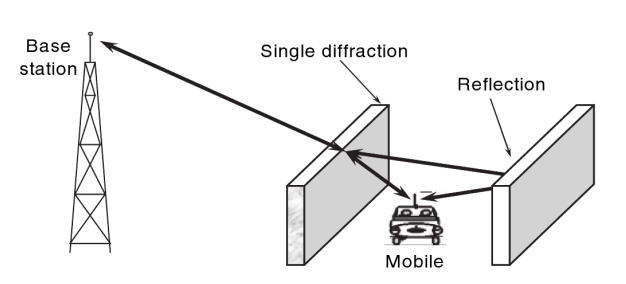
\includegraphics[scale=0.6]{images/difraccion-reflexion.png}
\caption{Interpretación física de los fenómenos difracción y reflexión. Imagen obtenida de (Aragón, 2008)}
\label{fig:shadowing}
\end{figure}

Un modelo comúnmente utilizado (no estadístico) que permite calcular la potencia de señal recibida está dado por la fórmula de transmisión definida por H. T. Friis, en donde sólo se considera la atenuación de la señal sobre el aire, descartando componentes fuera de la línea de visión (visibilidad directa entre antenas). Entonces, dadas dos antenas (asumiendo antenas isotrópicas), la relación entre la potencia de señal en la antena receptora $P_r$ y la potencia sometida a la antena transmisora $P_t$ esta dada por:

\begin{align}\label{eq:friis}
\frac{P_r}{P_t}=G_tG_r\left (\frac{\lambda}{4\pi d} \right)^2
\end{align}

siendo $G_t$ y $G_r$ las ganancias de las antenas transmisora y receptora, d la distancia entre las antenas y $\lambda$ la longitud de onda. En la ecuación \ref{eq:friis} puede notarse que la potencia recibida $P_r$ depende principalmente de la distancia $d$ entre el transmisor y el receptor. 

Al operar en 2.4 Ghz, en condiciones ideales (espacio libre o \textit{free space}), la atenuación (\textit{path loss})  sobre una distancia de 100 m es de 80.2 dB para un dispositivo Bluetooth Clase 1 (100 mW de potencia transmitida) y de 76.23 dB para un dispositivo Bluetooth Clase 2 (2.5 mW). En escenarios reales se producen mayores atenuaciones por los efectos descriptos anteriormente. En cuanto a la capacidad de detección de vehículos, se ha demostrado estadísticamente\cite{bakula2011probabilistic} que si el rango efectivo de detección es de 200 m (100 m en cada dirección), la probabilidad de hacer dos detecciones de un vehículo asciende a 94\%.  Sin embargo, a medida que disminuye el rango efectivo de un dispositivo sensor, la probabilidad de hacer una detección se verá altamente influenciada por la velocidad del vehículo, resultando en mayor cantidad de vehículos no detectados. 

\begin{figure}[!htp]
\centering
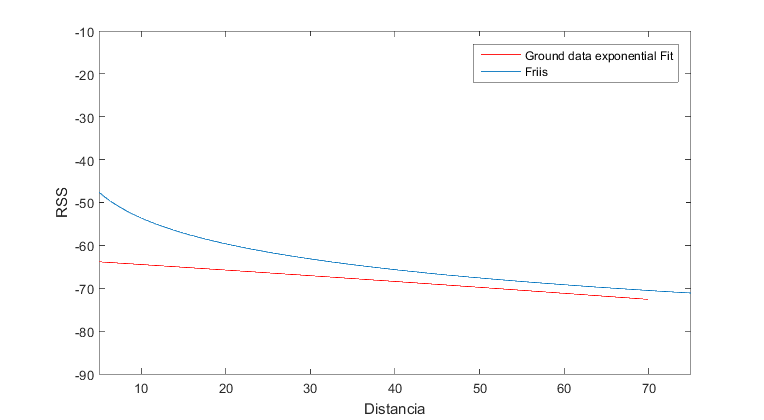
\includegraphics[scale=0.6]{images/friis-ground.png}
\captionsetup{width=.7\linewidth}
\caption{Comparación entre la ecuación de transmisión de Friis para un dispositivo transmisor Bluetooth Clase 2 con antena isotrópica dirigido a un receptor de antena 3 dBi, y una aproximación exponencial a partir de datos capturados por experimentación.}
\label{fig:friis-ground}
\end{figure}

En este trabajo se realizaron pruebas de campo con un vehículo con tecnología Bluetooth para caracterizar experimentalmente la pérdida de señal. La Figura \ref{fig:friis-ground} muestra la comparación entre una aproximación exponencial de los datos capturados y la pérdida de señal según el modelo de Friis. Naturalmente, la atenuación experimentada es mayor al modelo teórico debido a la ubicación del dispositivo Bluetooth en el interior del vehículo.

\section{Objetivo}
\label{sec:objetivo}

El objetivo es desarrollar un método de estimación de la red de tráfico a partir de información generada por distintos dispositivos utilizados en cada uno de los vehículos que circulan dentro de la red, los cuales pueden tener una aplicación específica para informar su posición (modo activo), o se puede considerar el registro de su posición a través de la detección de las señales Bluetooth (modo pasivo). Además, el método permitirá conocer el tiempo de viaje promedio dentro de la red y, para evaluar el sistema con un método de simulación, se deberá caracterizar la señal de radiofrecuencia de los dispositivos inalámbricos aplicando métodos de estimación de densidad de probabilidades, lo cual será detallado en el apartado \ref{ssec:kernel}. Finalmente, debido al alto costo que involucra plantear toda esta metodología en un caso real, se construirá una plataforma de simulación que permita evaluar los algoritmos desarrollados.

\section{Organización del documento}
\label{sec:documento}

El trabajo se estructura en 6 capítulos. En el capítulo 1 se presentó una breve introducción a la problemática en relación al tráfico vehicular, sus desafíos y un análisis de la situación actual en el país y el mundo. También se mencionan trabajos relacionados y los objetivos propuestos. En el capítulo 2, a través de definiciones y ejemplos concretos, se detalla el marco teórico que da lugar al Algoritmo de Viterbi, basado en Modelos Ocultos de Markov, una pieza fundamental del método de estimación propuesto. En el capítulo 3, se presentan los aspectos más importantes del método desarrollado, introduciendo conceptos relacionados a la solución de la problemática utilizando el Algoritmo de Viterbi (aplicado a tráfico vehicular). En el capítulo 4 se presentan los detalles de una plataforma para la estimación de tráfico vehicular, profundizando sobre una arquitectura preliminar preparada para la incorporación de mecanismos de simulación. Además, se detalla el método utilizado para caracterizar la señal de radiofrecuencia de dispositivos Bluetooth y cómo se utilizó para simular y detectar vehículos en viaje. En el capítulo 5 se realiza un análisis exhaustivo de los resultados de las estimaciones para GPS y Bluetooth, indicando la calidad de las estimaciones. Finalmente, en el capítulo 6 se hace una reflexión sobre el método desarrollado y los resultados obtenidos de los datos analizados, mencionando posibles mejoras y trabajos futuros. En el apéndice se incluyen gráficos y diagramas completos de la arquitectura y los procesos llevados a cabo en la caracterización Bluetooth.
